\subsection{Second peak}
\label{subsec:second_peak}

Modal parameters analysis applied to the second peak of the FRFs allows us to identify the natural frequency and the damping ratio of the second mode.
The identified parameters are reported in Table \ref{tab:second_peak}.

\begin{table}[H]
    \centering
    \begin{tabular}{lc}
        \hline
        $frequency_i [Hz]$ & ?? \\
        \hline
        $\xi_i [\%]$       & ?? \\
        \hline
    \end{tabular}
    \caption{Second peak modal parameters.}
    \label{tab:second_peak}
\end{table}

From a graphical point of view, the experimental and numerical FRFs are compared in Figure \ref{fig:second_peak}.

\begin{center}
    \huge{Plot to be replaced with the correct one.}
\end{center}

\begin{figure}[H]
    \centering
    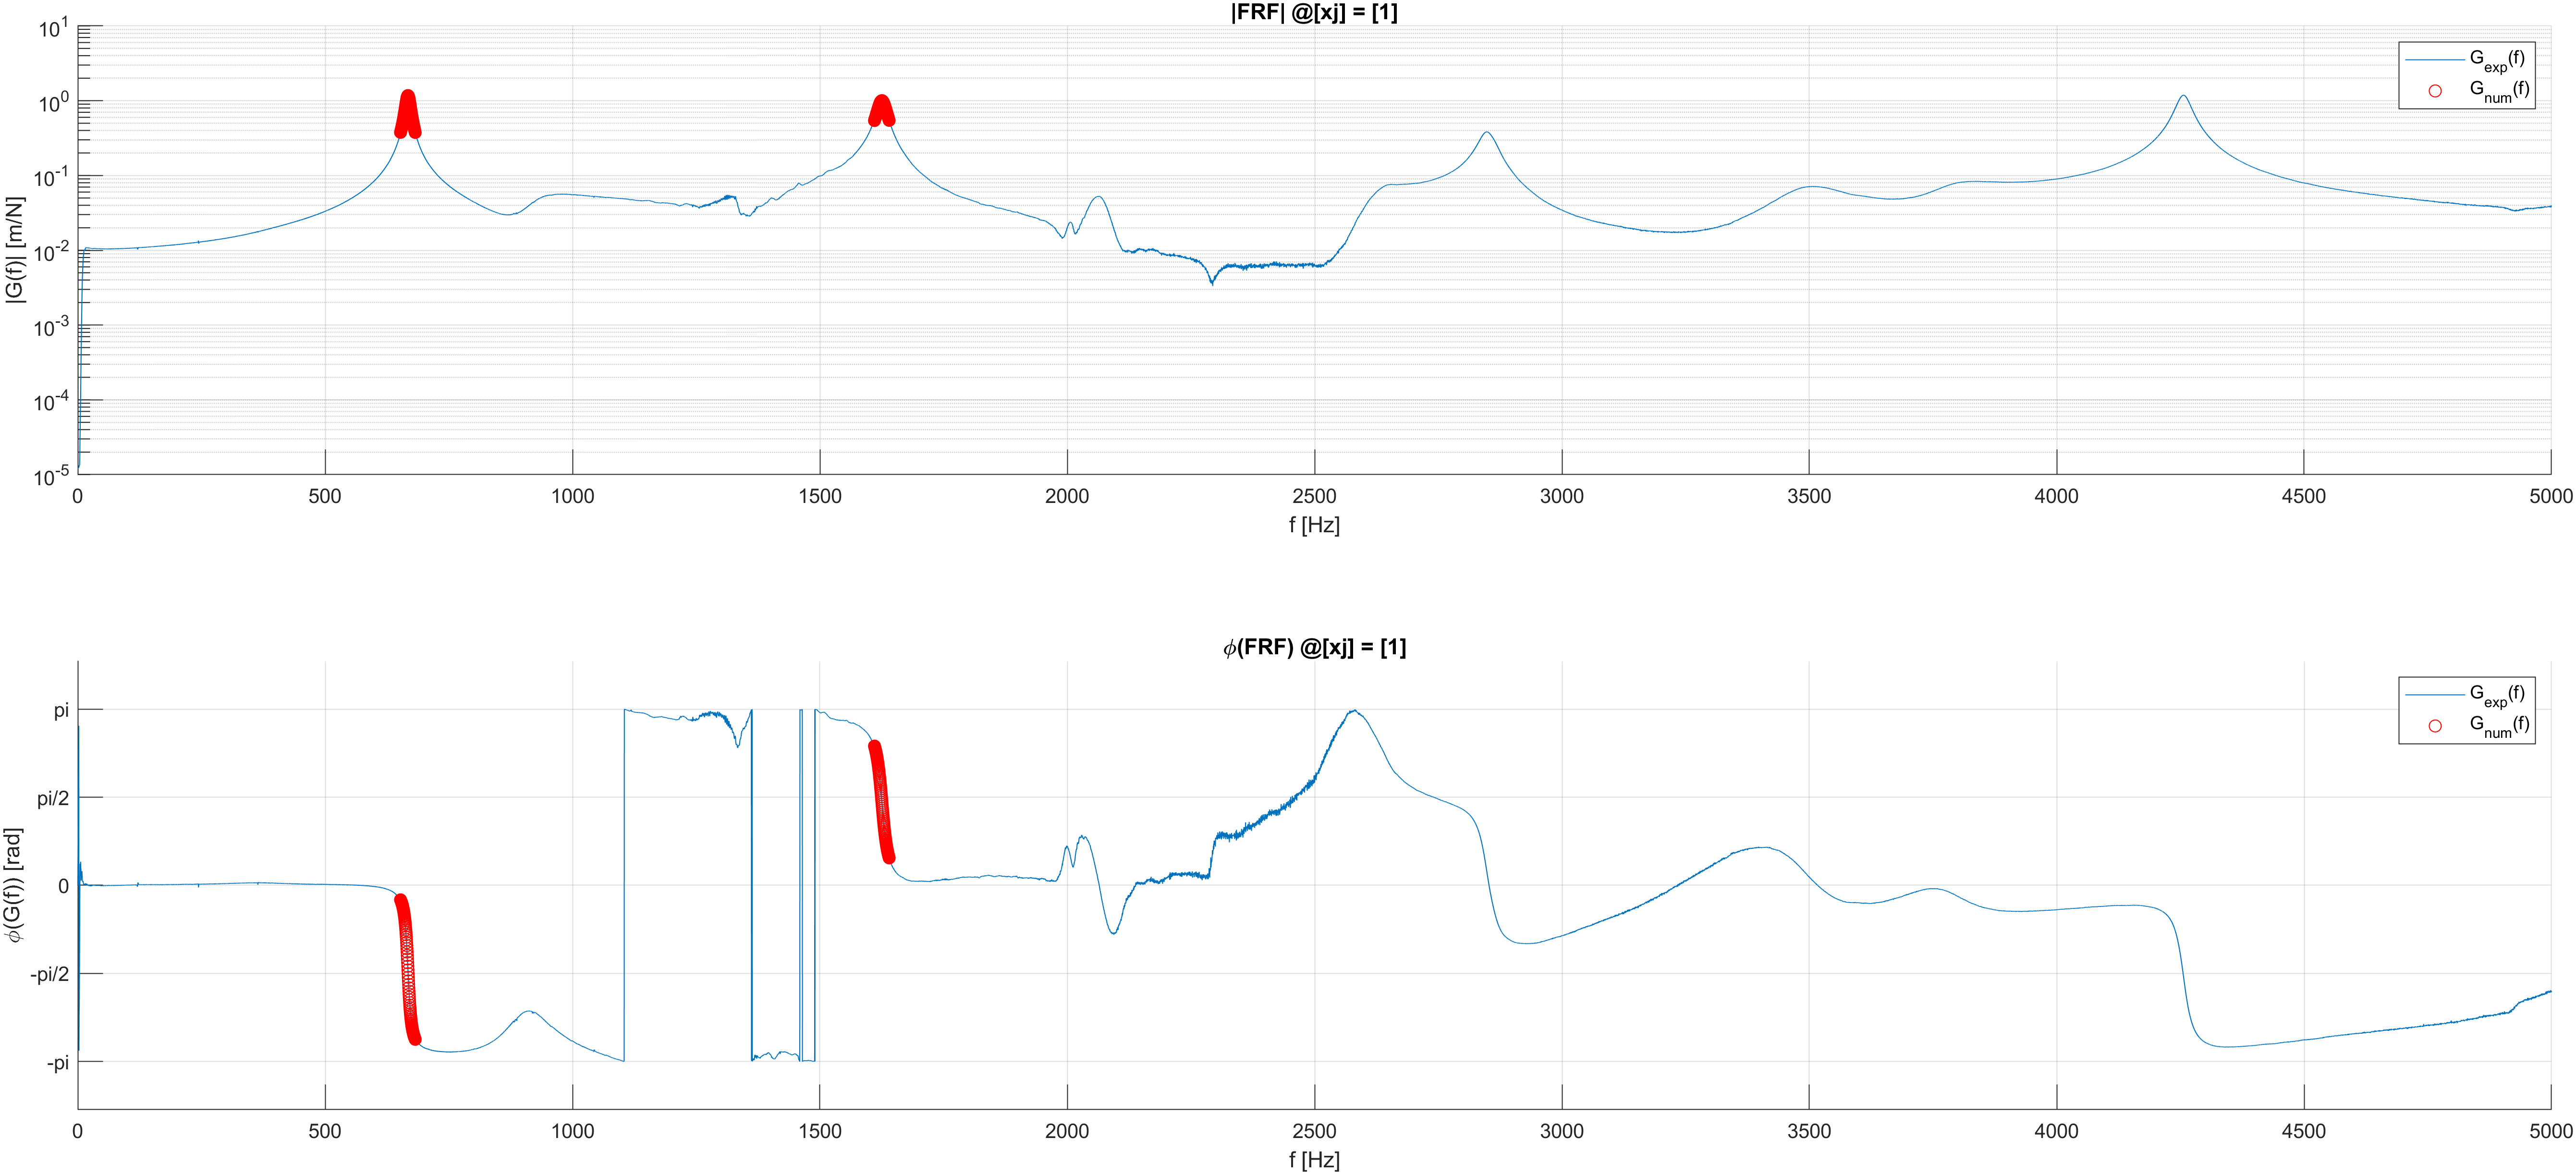
\includegraphics[width=\textwidth]{img/MATLAB/Part_B/Comparison_FRF_1.png}
    \caption{Second peak FRFs comparison.}
    \label{fig:second_peak}
\end{figure}
